\subsection{Conformidad con las preguntas de investigación}

Con respecto al cumplimiento de las preguntas de investigación definidas en la \autoref{subsubsec:rq-def}, se observó que la totalidad de los 22 estudios seleccionados aportó evidencia para responder la \textbf{RQ1}, lo que evidencia una cobertura completa de esta dimensión dentro del corpus analizado. Por su parte, 21 de los 22 estudios contribuyeron a responder la \textbf{RQ2}, indicando que esta temática también presenta una alta representación en la literatura considerada, aunque con un alcance ligeramente menor.

Estos resultados ponen de manifiesto una estrecha relación entre los objetivos de investigación planteados y los estudios finalmente incluidos en el mapeo sistemático, lo que respalda la pertinencia del proceso de selección aplicado. La distribución y el grado de solapamiento entre ambas preguntas de investigación se presentan en la \autoref{fig:grafica-venn-rqs}.

\begin{figure}[H]
	\centering
	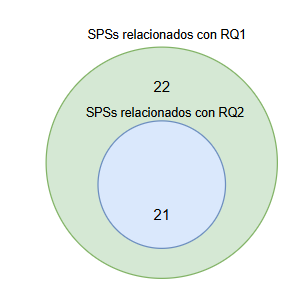
\includegraphics[width=0.4\textwidth]{mainmatter/II-desarrollo-metodologico/sms/imagenes/grafica-venn-rqs.png}
	\caption{Diagrama de los \acs{SPS}s relacionados con cada pregunta}
	\label{fig:grafica-venn-rqs}
\end{figure}
